\documentclass{beamer}
\beamertemplatenavigationsymbolsempty
\usecolortheme{beaver}
\setbeamertemplate{blocks}[rounded=true, shadow=true]
\setbeamertemplate{footline}[page number]
%
\usepackage[utf8]{inputenc}
\usepackage[english,russian]{babel}
\usepackage{amssymb,amsfonts,amsmath,mathtext}
\usepackage{subfig}
\usepackage[all]{xy} % xy package for diagrams
\usepackage{array}
\usepackage{multicol}% many columns in slide
\usepackage{hyperref}% urls
\usepackage{tabularx}
\usepackage{hhline}%tables
% Your figures are here:
\graphicspath{ {fig/} {../figures/} }

%----------------------------------------------------------------------------------------------------------
\title[\hbox to 56mm{Оптимальные методы оптимизации первого порядка с относительным шумом}]{Оптимальные методы оптимизации первого порядка с относительным шумом}
\author[Д.\,Н. Рубцов]{Денис Николаевич Рубцов}
\institute{Московский физико-технический институт}
\date{\footnotesize
\par\smallskip\emph{Курс:} Автоматизация научных исследований\par (практика, В.\,В.~Стрижов)/Группа 105
\par\smallskip\emph{Эксперт:} к.ф.-м.н. Э.\,А.~Горбунов
\par\smallskip\emph{Консультант:} Н.\,М.~Корнилов
\par\bigskip\small 2024}
%----------------------------------------------------------------------------------------------------------
\begin{document}
%----------------------------------------------------------------------------------------------------------
\begin{frame}
\thispagestyle{empty}
\maketitle
\end{frame}
%-----------------------------------------------------------------------------------------------------
\begin{frame}{Цель исследования}
     \begin{block}{Цели}
     \begin{itemize}
         \item разработать оптимальные алгоритмы оптимизации первого порядка, в которых градиенты известны лишь с некоторой относительной погрешностью
         \item исследовать скорость сходимости этих алгоритмов
     \end{itemize}
     \end{block}

 \end{frame}
%-----------------------------------------------------------------------------------------------------
\begin{frame}{Оптимизация первого порядка}
\begin{columns}[c]
\column{0.45\textwidth}
\begin{block}{Решается задача}
\[x_{\star} = \arg \min_{x \in \mathbf{R}^d} f(x)\]
\[f(x) \in \mathcal{F}\]
\end{block}
\begin{block}{Анализ наихудшего случая}
\[ \max_{f \in \mathcal{F}, \ (x_t)_{t \le T} \in (\mathbf{R}^d)^{T+1}} P(f, (x_t)_{t \le T})\]
\[\text{s.t.} 
\begin{cases}
x_0 \in \mathcal{N}(x_{\star}) \\
(x_t)_{t \le T} = \mathcal{A}(f, T, x_0)
\end{cases}
\]
\end{block}
%\begin{block}{Неточный градиент}
%\[\mathcal{O}^{(f)}(x) = \widetilde{\nabla} f(x)\]
%\end{block}
\column{0.55\textwidth}
\begin{table}[h!]
\centering
 \begin{tabular}{||p{1.8 cm} p{3 cm}||} 
 \hline

 $\mathcal{F}$ & некоторый класс функций  \\ 
 \hline
 $\mathcal{F}_{\mu, L}$ & класс $\mu$-сильно выпуклых $L$-гладких функций  \\ 
 \hline
 $f$ & исследуемая функция  \\
 \hline
 $x_{\star}$ & точка минимума  \\
 \hline
 $x_0$ & начальная точка  \\
 \hline
 $\mathcal{O}^{(f)}$ & оракул  \\ 
 \hline
 $\mathcal{A}$ & алгоритм  \\
 \hline
 $(x_t)_{t \le T}$ & последовательность точек  \\
 \hline
 $T$ & число итераций  \\ 
 \hline
 $P(f, (x_t)_{t \le T})$ & метрика точности  \\[1ex] 
 \hline
 \end{tabular}
\end{table}
\end{columns}
\end{frame}

%-----------------------------------------------------------------------------------------------------
\begin{frame}{Постановка задачи}
\begin{columns}[c]
\column{0.5\textwidth}
\begin{block}{Решается задача}
\[x_{\star} = \arg \min_{x \in \mathbf{R}^d} f(x)\]
\[f(x) \in \mathcal{F}_{\mu, L}\]
\end{block}
\begin{block}{Жадный алгоритм}
\[ \max_{f \in \mathcal{F}_{\mu, L}, \ (x_t)_{t \le T} \in (\mathbf{R}^d)^{T+1}} f(x_t) - f_{\star}\]
\[\text{s.t.} 
\begin{cases}
x_0 \in U_R(x_{\star}) \\
(x_t)_{t \le T} = \text{span} \{ x_t, (\mathcal{O}^{(f)}_{t})_{t \le T} \}
\end{cases}
\]
\end{block}

\column{0.5\textwidth}
\begin{block}{Неточный градиент}
\[\mathcal{O}^{(f)}(x) = \widetilde{\nabla} f(x)\]
\[\|\widetilde{\nabla} f(x) - \nabla f(x)\|_2 \leq \hat{\varepsilon} \|\nabla f(x)\|_2 \\ \quad \forall \hat{\varepsilon} \in [0, 1].\]
\end{block}

\begin{block}{Гипотеза}
$f(x_{t}) - f(x_{\star}) \le q^t (f(x_0) - f(x_{\star})$
\begin{table}[h!]
\centering
 \begin{tabular}{||c | c||} 
 \hline
 GD & NAG, HB\\ 
 \hline
  $q \sim \frac{\mu}{L}$ & $q \sim \sqrt{\frac{\mu}{L}}$ \\ 
 \hline
 \end{tabular}
\end{table}
\begin{center}
 $q \sim (\frac{\mu}{L})^{g(\varepsilon)}$   
\end{center}
\end{block}
\end{columns}
\end{frame}

%-----------------------------------------------------------------------------------------------------
\begin{frame}{Поясняющие картинки}
\begin{columns}[c]
\column{0.5\textwidth}
\begin{figure}
\includegraphics[width=1.0\textwidth]{Interpolation.png}
    \caption{Плодотворные идеи интерполяции в PEP. Можно ли по значениям точек, значениям точек и производным в этих точках восстановить функцию нужного класса?}
\end{figure}
\column{0.5\textwidth}
\begin{figure}
\includegraphics[width=1.0\textwidth]{InterpolateCvx.png}
    \caption{Плодотворные идеи интерполяции в PEP. Ответ - да. Можно брать максимум значений красных пунктирных линий (поточечный максимум)}
\end{figure}
\end{columns}
\end{frame}
%-----------------------------------------------------------------------------------------------------
\begin{frame}{Вычислительные эксперименты}
\begin{center}
$\tau_t = f(x_{t}) - f(x_{\star}) \le q^t (f(x_0) - f(x_{\star}) \Rightarrow \log{\tau_t} \sim t$ \\

 $q \sim (\frac{\mu}{L})^{g(\varepsilon)}$ \\ 
 
 $\log{q} \sim g(\varepsilon) \log{\mu}$
\end{center}

\begin{columns}[c]
\column{0.5\textwidth}
\begin{figure}
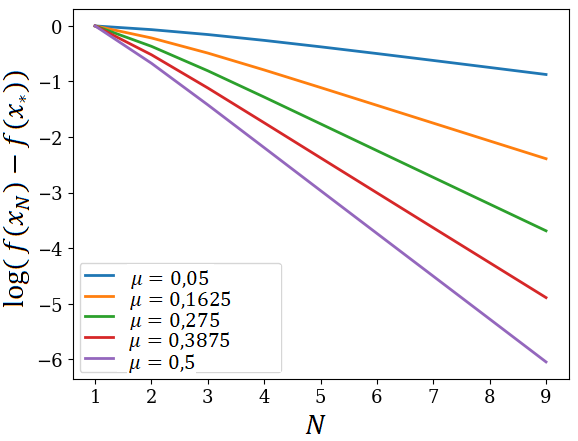
\includegraphics[width=1.0\textwidth]{linear_convergence.png}
    \caption{График зависимости лонарифма невязки от номера итерации $\log{\tau_t} \sim t$ при $\varepsilon = 0.5$. Доказывает линейную сходимость.}
\end{figure}
\column{0.5\textwidth}
\begin{figure}
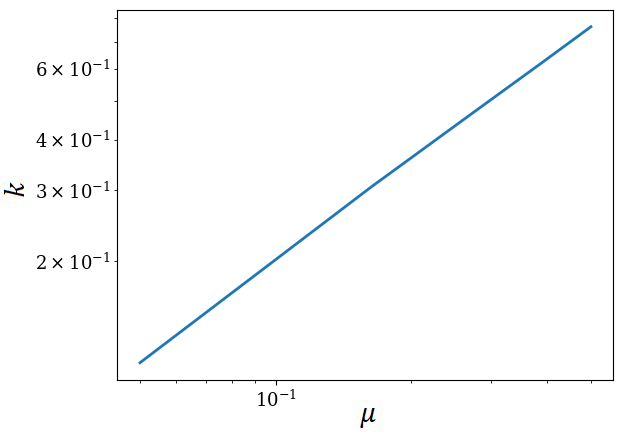
\includegraphics[width=1.0\textwidth]{q_mu_grqph.png}
    \caption{График зависимости $q(\mu)$ при $\varepsilon = 0.5$ в лог-лог-масштабе. Показывает, что степень сходимости зависит лишь от шума}
\end{figure}
\end{columns}
\end{frame}
%-----------------------------------------------------------------------------------------------------
\begin{frame}{Основной результат вычислительных экспериментов}
\begin{center}
 $q \sim (\frac{\mu}{L})^{g(\varepsilon)}$ \\ 
\end{center}
\begin{figure}
\includegraphics[width=0.6\textwidth]{degree_of_convergence.png}
    \caption{График зависимости $g(\varepsilon)$. При нулевом шуме, сходимость как у ускоренных методов (NAG, HB). При больших шумах сходимость как у GD}
\end{figure}
\end{frame}



%-----------------------------------


%----------------------------------------------------------------------------------------------------------

%----------------------------------------------------------------------------------------------------------

%----------------------------------------------------------------------------------------------------------
\begin{frame}{Заключение}
     \begin{block}{Результаты}
     \begin{itemize}
         \item предложена гипотеза сходимости оптимального (жадного) алгоритма оптимизации первого порядка в случае, когда градиенты известны лишь с некоторой погрешностью
         \item гипотеза доказана численно
     \end{itemize}
     \end{block}
     \begin{block}{Планы}
     \begin{itemize}
         \item теоретическое доказательсто полученных экспериментальных результатов
     \end{itemize}
     \end{block}
 \end{frame}
%----------------------------------------------------------------------------------------------------------
%-----------------------------------

\begin{frame}{Литература}

\begin{itemize}
 \item Baptiste Goujaud, Aymeric Dieuleveut, and Adrien Taylor. On fundamental proof structures in first-order
optimization. In 2023 62nd IEEE Conference on Decision and Control (CDC), pages 3023–3030. IEEE,
2023.
 \item Nikita Kornilov, Eduard Gorbunov, Mohammad Alkousa, Fedor Stonyakin, Pavel Dvurechensky, and Alexander Gasnikov. Intermediate gradient methods with relative inexactness. arXiv preprint arXiv:2310.00506, 2023
 \item Adrien B Taylor. Convex interpolation and performance estimation of first-order methods for convex optimization. PhD thesis, Catholic University of Louvain, Louvain-la-Neuve, Belgium, 2017
 \item Adrien B Taylor, Julien M Hendrickx, and Fran ̧cois Glineur. Smooth strongly convex interpolation and exact worst-case performance of first-order methods. Mathematical Programming, 161:307–345, 2017.
\end{itemize}

\end{frame}

\end{document} 
